%!TEX program = xelatex
\documentclass[11pt,oneside]{book}
\usepackage{fontspec, xunicode, xltxtra}  
\setmainfont{Hiragino Sans GB}  
%%%%%%%%%%%%% Geometry
\usepackage[a4paper,left=2.5cm,right=2.5cm, bottom=2.5cm,top=2.5cm]{geometry}

%%%%%%%%%%%%%%% Les paquets

\usepackage[english]{babel}
\usepackage[palette=munch]{nexus}
\usepackage{verbatim}
\usepackage{listings} 

%%%%%%%%%%%%%%%% hyperref
\usepackage{lipsum}
\usepackage{graphicx}
\XeTeXlinebreaklocale "zh"
\XeTeXlinebreakskip = 0pt plus 1pt
\usepackage[verbose]{hyperref}
\hypersetup{ 
    hidelinks
}
\setlength{\XeTeXLinkMargin}{-1pt}


\begin{document}

\pagestyle{empty}

\definecolor{plop}{HTML}{4D7186}
\begin{textblock}{1}(0,0)
    \noindent\textcolor{plop}{\rule{\paperwidth}{.55\paperheight}}
\end{textblock}


\begin{textblock}{1}(0,.55)
    \noindent\textcolor{black}{\rule{\paperwidth}{.45\paperheight}}
\end{textblock}


\begin{textblock}{1}(.1,.09)
    \noindent{\fontsize{24.88}{2}\selectfont
        \bfseries\textcolor{white}{Report for}}
\end{textblock}

\begin{textblock}{1}(.1,.15)
    \noindent {\fontsize{24.88}{2}\selectfont
    \bfseries\textcolor{white}{Digital Image Processing}}
\end{textblock}

% \begin{textblock}{1}(.1,.21)
%     \noindent{\fontsize{30}{2}\selectfont
%         \bfseries\textcolor{white}{for \LaTeX}}
% \end{textblock}

\begin{textblock}{1}(.1,.45)
    \noindent {\fontsize{20.74}{2}\selectfont
        \bfseries\textcolor{white}{Fanyong Xue}}
\end{textblock}



\begin{textblock}{.9}(.05,.56)
    \begin{flushright}
        \noindent {\fontsize{20.74}{2}\selectfont
            \bfseries\textcolor{orange}{version 1.1}}
    \end{flushright}
\end{textblock}


\begin{textblock}{.45}(.5,.82)
    \begin{center}
        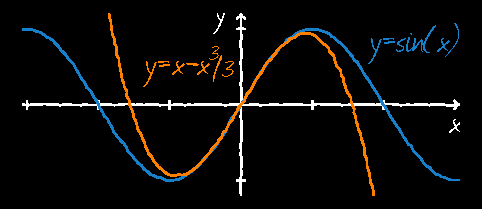
\includegraphics[width=.45\paperwidth]{dlsin}
    \end{center}
\end{textblock}

\begin{textblock}{.4}(.05,.65)
    \begin{center}
        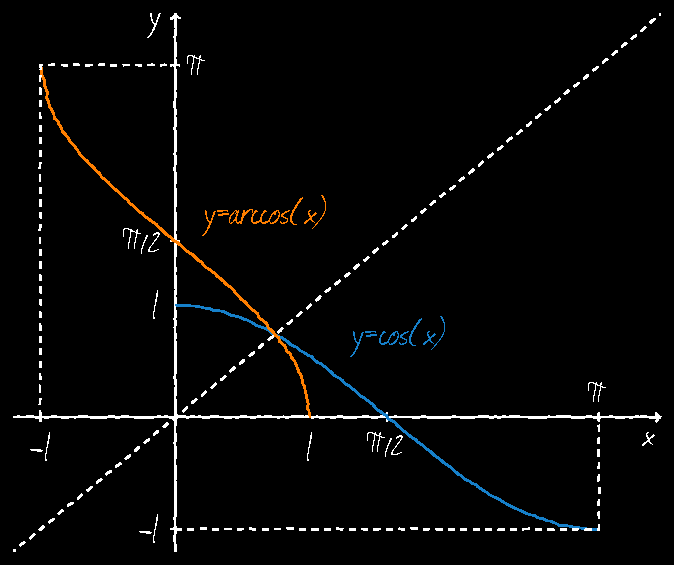
\includegraphics[width=.4\paperwidth]{arccos}
    \end{center}
\end{textblock}


\begin{textblock}{.6}(.05,.6)
    \noindent {\fontsize{20.74}{18}%
    \textcolor{white}{$\displaystyle(a+b)^n = \sum_{k=0}^n 
                \binom{n}{k} a^kb^{n-k}$}}
\end{textblock}


\begin{textblock}{.4}(.4,.77)
    \noindent {\fontsize{17.28}{18}%
    \textcolor{white!80}{$\displaystyle 
                \neg (p\vee q) \equiv (\neg p)\wedge (\neg q)$}}
\end{textblock}

\begin{textblock}{.4}(.1,.93)
    \noindent {\fontsize{14.4}{18}%
    \textcolor{white!50}{$\displaystyle 
                \binom{n}{k} = \frac{n!}{k!(n-k)!}$}}
\end{textblock}


\begin{textblock}{.6}(.5,.69)
    \noindent {\fontsize{17.28}{18}%
    \textcolor{white!10}{$\displaystyle 
                \zeta_k = |a|^{1/n} \mathrm{e}^{i(\mathrm{arg}(a)+2k\pi)/n}$}}
\end{textblock}


\begin{textblock}{.3}(.75,.73)
    \noindent {\fontsize{17.28}{18}%
    \textcolor{white!10}{$\displaystyle \mathrm{e}^{i\pi}+1=0$}}
\end{textblock}



\null\newpage\pagestyle{nexus}

\tableofcontents

\chapter{Histogram Equalization}

\section{OverView}
(a) Write a computer program for computing the histogram of an image.

(b) Implement the histogram equalization technique.

(c) Your program must be general to allow any gray-level image as its input.

As a minimum, your report should include the original image, a plot of its histogram, a plot of the transformation function, the enhanced image, and a plot of its histogram.
\section{Generate the Histogram}
\subsection{Function}
Generating the histogram of an image using flowwing function:\\
\begin{center}
$H(i) = the\ number\ of\ pixel\ whose\ value\ euquals\ to\ i$
\end{center}
\subsection{Histogram}
The histogram pictures of Fig1.jpg and Fig2.jpg are listed as follows:
\begin{figure}[!htb]
   \centering  
   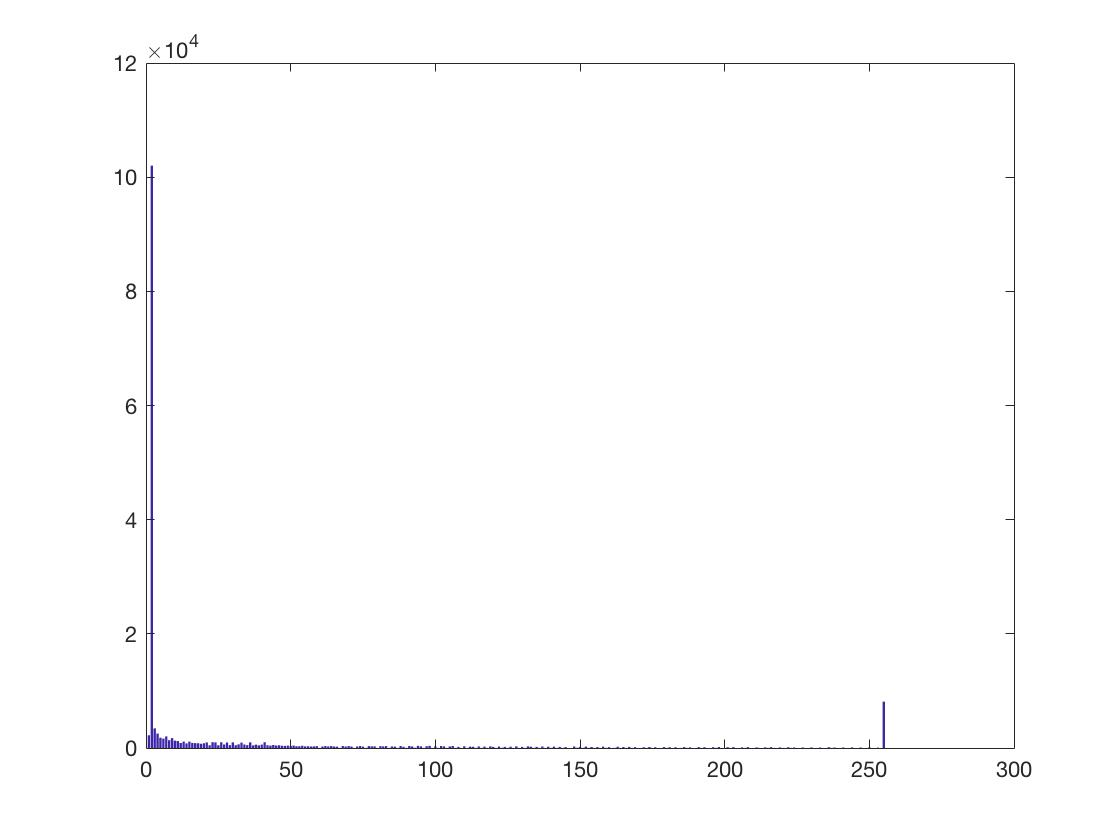
\includegraphics[width=1.0\textwidth]{images/1/histogram1.jpg}
   \caption{Histogram of fig1.jpg}  
\end{figure}
\begin{figure}[!htb]
   \centering  
   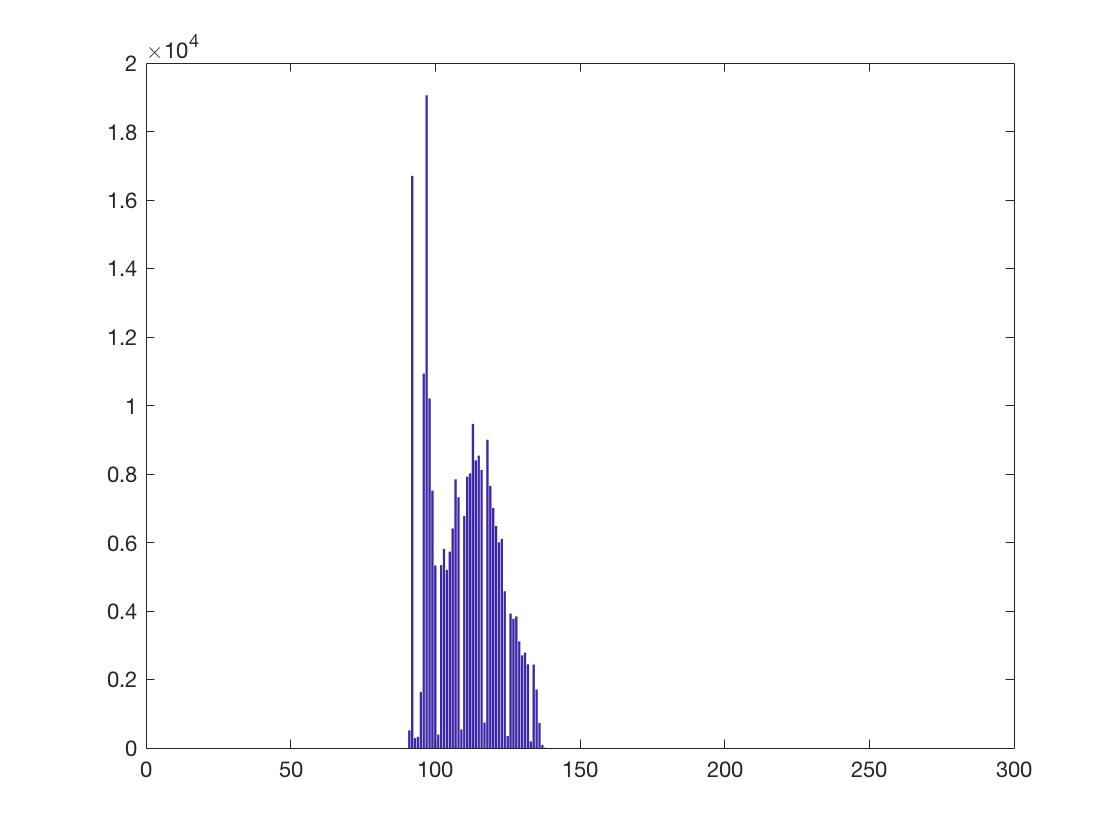
\includegraphics[width=1.0\textwidth]{images/1/histogram2.jpg}
   \caption{Histogram of fig2.jpg}  
\end{figure}

\section{Transfer Function}
\subsection{Implement the Histogram Equalization Technique}
We use those functions to calculate the histogram equalization:\\
\begin{center}
$L=Max(image(r,c))\ \forall r \in [1,rows]\ and\ \forall c \in [1,cols]$\\
$s(r_k) = L*T(r_k) = L*\sum_{j=0}^kP_r(r_j)=L*\sum_{j=0}^k\frac{n_j}{n}$
\end{center}
\newpage
\subsection{Transfer Function}
The transfer function of Fig1.jpg and Fig2.jpg are listed as follows:
\begin{figure}[!htb]
   \centering  
   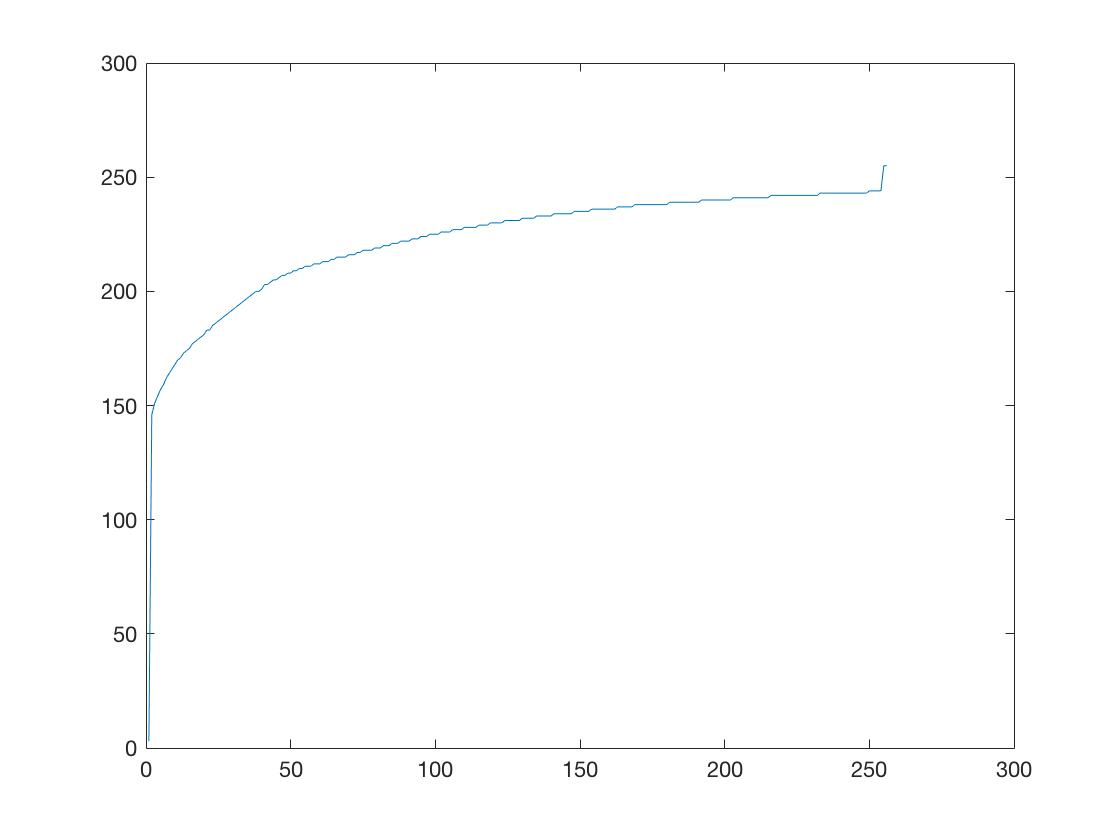
\includegraphics[width=0.8\textwidth]{images/1/transfer_f1.jpg}
   \caption{Transfer Function of fig1.jpg}  
\end{figure}
\begin{figure}[!htb]
   \centering  
   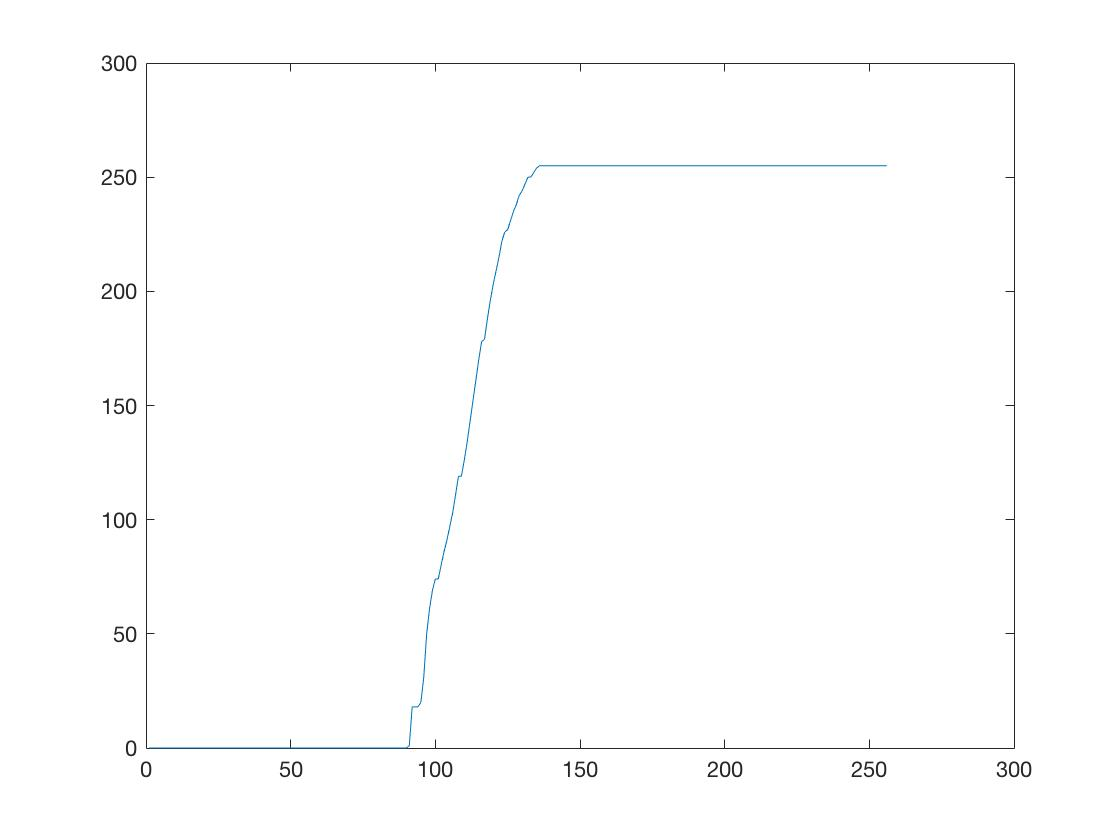
\includegraphics[width=0.8\textwidth]{images/1/transfer_f2.jpg}
   \caption{Transfer Function of fig2.jpg}  
\end{figure}
\section{Enhanced Images}
\subsection{Enhanced Function}
We use the function\\
\begin{center}
$New\ Image(r,c) = Transfer\ Function(image(r,c))\ \forall r \in [1,rows]\ and\ \forall c \in [1,cols]$
\end{center}
to enhance the original images. 
\subsection{Enhanced Images}
The original images and enhanced images and its histogram are listed as follows.
\begin{figure}[!htb]
   \centering  
   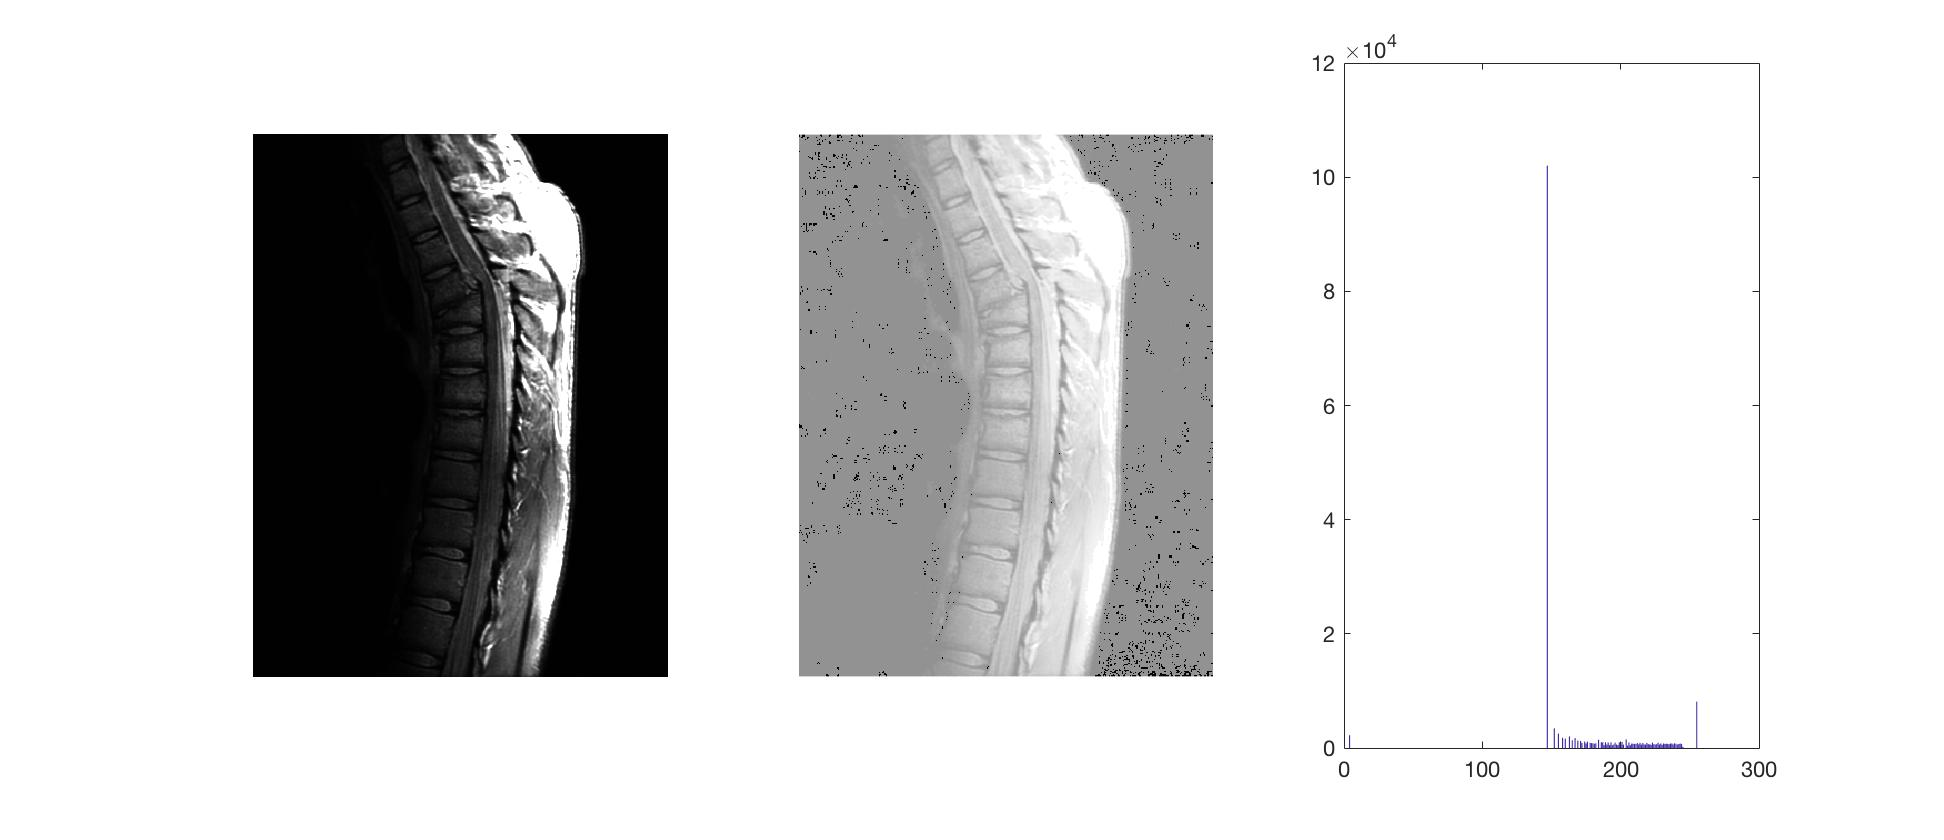
\includegraphics[width=1.0\textwidth]{images/1/image1.jpg}
   \caption{original image and enhanced image and its histogram of fig1.jpg}  
\end{figure}
\begin{figure}[!htb]
   \centering  
   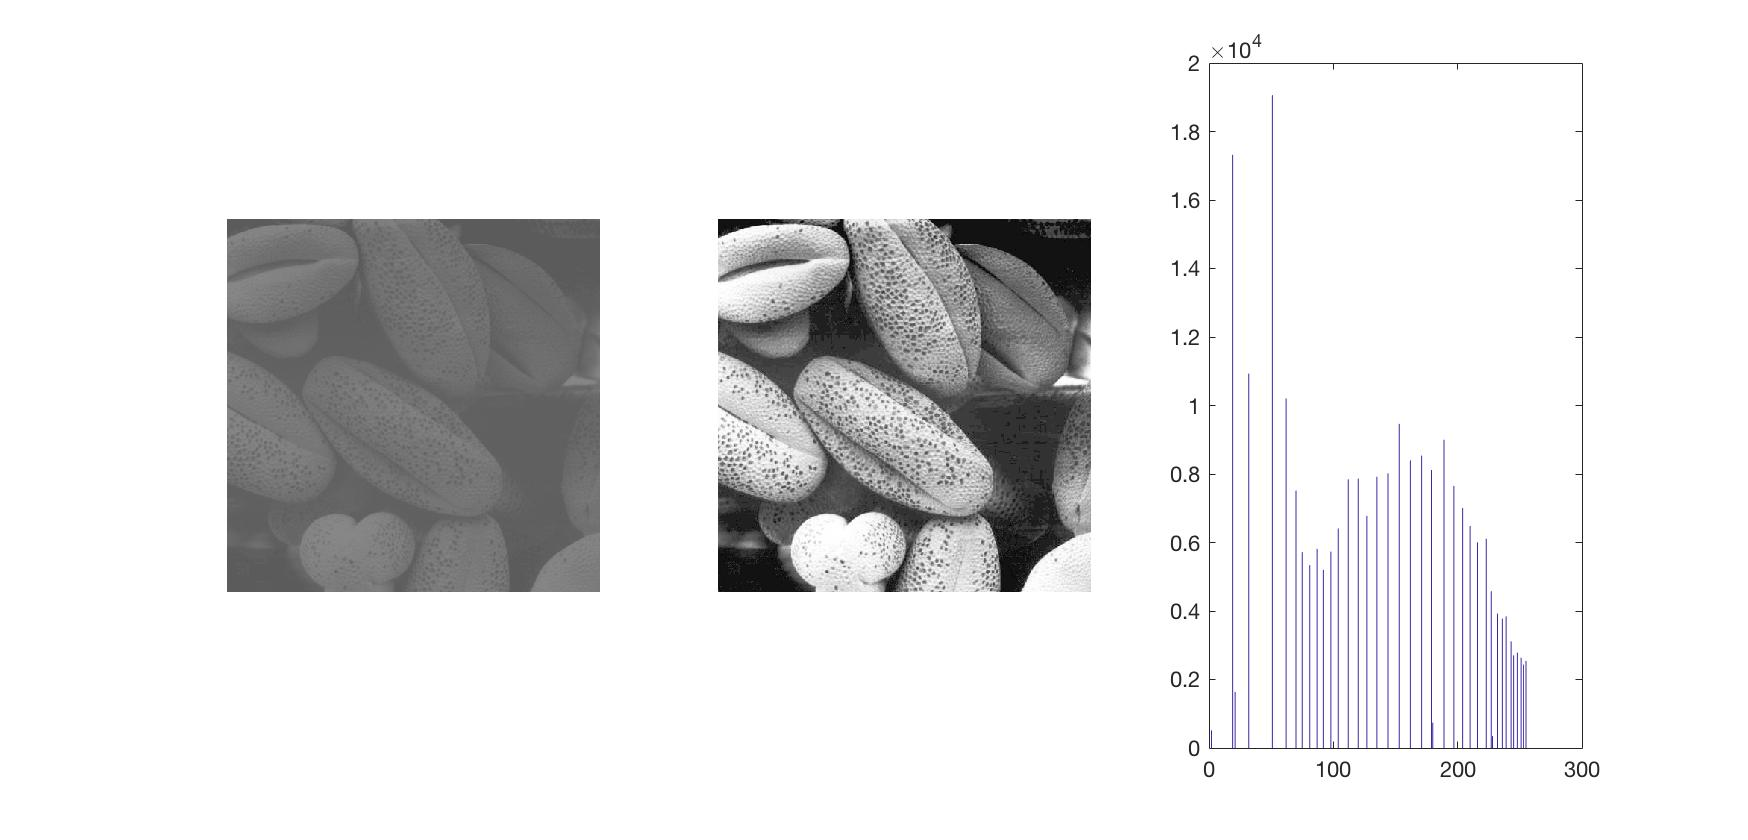
\includegraphics[width=1.0\textwidth]{images/1/image2.jpg}
   \caption{original image and enhanced image and its histogram of fig2.jpg}  
\end{figure}





\chapter{Combining spatial enhancement methods}
\section{OverView}
   Implement the image enhancement task of Section 3.7 (Fig 3.43, page 171). The image to be enhanced is skeleton\_orig.tif. You should implement all steps in Figure 3.43. (You are encouraged to implement all functions by yourself, not to directly use Matlab functions such as imfilter or fspecial.)



\chapter{Filtering in frequency domain}
Implement the ideal, Butterworth and Gaussian lowpass and highpass filters and compare the results under different parameters using the image characters\_test\_pattern.tif (this image file can be found at the ftp server ftp://ftp.cs.sjtu.edu.cn:990/lu-ht/DIP/images) as the test pattern.

\section{This is a section}
\subsection{This is a subsection}
\lipsum[1-1]
\subsection{This is a subsection}
\lipsum[1-2]

\chapter{Generating different types of noise and comparing different noise reduction methods}
\section{OverView}
In this problem, you are required to write a program to generate different types of random noise (Uniform, Gaussian, Rayleigh, Gamma, Exponential and Impulse, first started from the uniform noise and then use some functions to convert the uniform noise to Gaussian, Rayleigh, Gamma and Exponential; Impulse noise is generated in a different way, consulting the textbook and some other references) and then add these noises to the test patter image Fig0503(original\_pattern).tif to compare the visual results of the noisy images.

Add some of these noises to the circuit image Circuit.tif (images can be found at ftp://ftp.cs.sjtu.edu.cn:990/lu-ht/DIP/images) and investigate the noise reduction results using different mean filters and order statistics filters as the textbook did at pages 344-352 (Pages 322-329 in the electronic version of the textbook).

\section{This is a section}
\subsection{This is a subsection}
\lipsum[1-1]
\subsection{This is a subsection}
\lipsum[1-2]

\chapter{Image restoration}
\section{OverView}


\section{This is a section}
\subsection{This is a subsection}
\lipsum[1-1]
\subsection{This is a subsection}
\lipsum[1-2]


%%%%%%
\begin{appendices}
\chapter{Codes}
\section{Problem1}

\begin{lstlisting}[numbers=left, numberstyle=\tiny,keywordstyle=\color{blue!70},commentstyle=\color{red!50!green!50!blue!50},frame=shadowbox, rulesepcolor=\color{red!20!green!20!blue!20}] 
% Problem 1
% by Xue Fanyong
% Student ID:515030910443
% Histogram Equalizatio

%% main part
image1 = imread('Image Path/Fig1.jpg');
image2 = imread('Image Path/Fig2.jpg');

[histogram1,histogram_e1,transfer_f1,image_e1] = 
histogram_equalization(image1);
[histogram2,histogram_e2,transfer_f2,image_e2] = 
histogram_equalization(image2);

plot_data(image1,image_e1,histogram1,histogram_e1,transfer_f1);
plot_data(image2,image_e2,histogram2,histogram_e2,transfer_f2);

%% functions part

% get histogram of image
% image: get histogram of it
% histogram: the histogram of image
function histogram = get_histogram(image)
    histogram = zeros(256,1);
    [row,col]=size(image);
    for r = 1:row
        for c = 1:col
            gray = image(r,c);
            histogram(gray+1)=histogram(gray+1)+1;
        end
    end
end

% do the histogram_equalization for image
% image: do histogram_equalization for it
% histogram: original histogram; histogram_e: 
% histogram after histogram
% equalizatio; transfer_f: transfer function; 
% image_e: image after histogram
% equalizatio
function [histogram,histogram_e,transfer_f,image_e] = 
histogram_equalization(image)
    [row,col]=size(image);
    transfer_f = zeros(256,1);
    histogram = get_histogram(image);
    transfer_f(1) = 256*histogram(1)/(row*col);
    
    for i = 2:256
        transfer_f(i) = transfer_f(i-1)+255*histogram(i)/(row*col);
    end
    transfer_f = round(transfer_f);
    
    image_e = image;
    for r = 1:row
        for c = 1:col
            image_e(r,c)=transfer_f(image(r,c)+1);
        end
    end
    histogram_e = get_histogram(image_e);
end

% plot data
% image:original image; image_e: 
% image after histogram equalizatio; 
% histogram: original histogram; 
% histogram_e: histogram after histogram equalizatio;
% transfer_f: transfer function
function plot_data(image,image_e,histogram,histogram_e,transfer_f)
    figure();
    subplot(2,3,1);
    imshow(image);
    title("Original Image");
    subplot(2,3,2);
    imshow(image_e);
    title("Image(Histogram Equalization)");
    subplot(2,3,3);
    bar(histogram);
    title("Histogram");
    subplot(2,3,4);
    bar(histogram_e);
    title("Histogram(Equalization)");
    subplot(2,3,5);
    plot(transfer_f);
    title("Transfer Funciton");
end

\end{lstlisting}


\section{This is a section}


\end{appendices}

\end{document}

